\chapter{Storage System Design} \label{chapWhDesign}

This section is about warehouse design, i.e. the design from scratch or the redesign of an existing storage system ~\cite{Ashayeri1985, VanGils2017b} . This activity involves many decision problems belonging to different classes. In practice, these problems are approached in sequence, enlarging the focus of the decision from stock keeping units (SKUs), to storage areas to handling areas ~\cite{Accorsi2012, Baker2009, Dotoli2015, Park1989, Tufano2019,Yoon1996}. Figure \ref{fig_warehouse_design} identifies the hierarchical procedure used in this chapter, according to the definition of logistics problems introduced in \ref{secDecisionPatterns}. SKU are the parts stored within the storage system. Same SKUs has the same properties (e.g. id, weight, volume, package). Storage areas are a set of storage locations of the warehouse having a similar storage technology (e.g. served by forklifts, automated guided vehicle (AGV), automated storage and retrieval systems (AS/RS)). Handling areas are sets of storage areas, processing areas (e.g. packing, quality control, inbound and outbound areas), and edges (i.e. aisles connecting all these areas).

% INSERT fig_warehouse_design
\begin{figure}[hbt!]
\centering
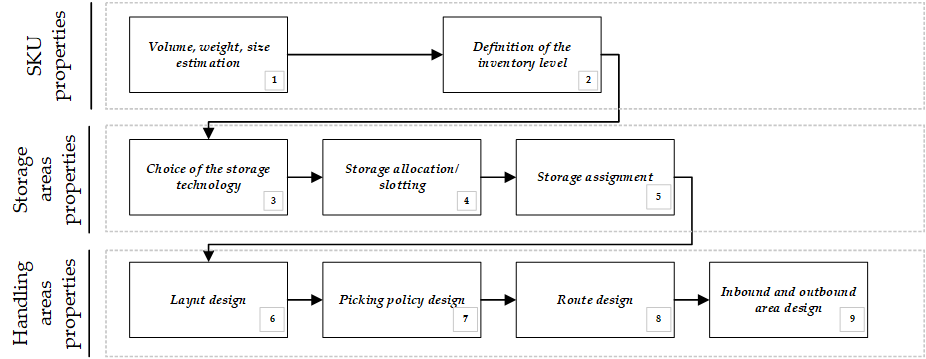
\includegraphics[width=0.9\textwidth]{SectionWarehouses/design_figures/fig_warehouse_design.png}
\captionsetup{type=figure}
\caption{Hierarchical procedure for storage system design.}
\label{fig_warehouse_design}
\end{figure}

The hierarchical procedure identifies nine decision problems:
\begin{enumerate}
    \item The estimation of weights and sizes for all the SKUs of the storage system;
    \item The definition of the inventory level for each SKU;
    \item The choice of the storage technology for each set of SKUs;
    \item The allocation of storage space to SKUs;
    \item The assignment (also known as “slotting”) of SKUs to storage locations;
    \item The design of the layout of a handling area;
    \item The definition of the picking policies (e.g. single order/batching/zoning);
    \item The definition of the routing policy (i.e. returns; traversal);
    \item The design of the inbound and outbound areas.

\end{enumerate}

The following paragraphs introduce model- and data-driven methods to address these problems.

\section{Weight and size estimation (P1)}
The knowledge of the features of the SKUs is the first step to design a storage system adequately. It may appear evident that companies must know everything about their parts. Nevertheless, the SKU master file of a warehouse management system (WMS) is easily full of null values. The most important indicator to design a storage system is the volume of its SKUs; this value is often unknown due to the labour-intensive activity to measure the dimensions of thousands of SKUs. In practice, a warehouse designer needs to know the size (i.e. length, height and width), and the weight of an SKU.

\subsection{Model-driven methods (D2)}
When sizes and weights are unknown for all the SKUs of a storage system, on-field measurement is the only possibility to start generating this data. A scale is used to measure the weight; the length, height, and width of an SKU are used to define its volume. When dealing with the measurement of the volume of the SKUs of an existing storage system, an approximate procedure exist. Let $v_i$ be the volume of SKU $i$ to measure. We estimate the volume $v_i$ by using  $\widehat{v_i}=\frac{1}{card(j:n_{ij}>0)}\ \sum_{j:n_{ij>0}}\left[\frac{V_j\ \eta_j}{n_{ij}}\right]$ where  $\eta_j\in[0,1]$ is the percentage saturation of each storage location $j$, and $n_{ij}$ is the number of SKUs $i$ stored in each location $j$. $V_j$ is the volume of the storage location $j$. This way, it is possible to measure a single storage location $j$, to observe the storage locations to estimate $\eta_j$, and to consider the number of SKUs $n_{ij}$ obtained, for example, from the inventory of the WMS. This procedure is approximated but faster than measuring thousands of SKUs and it provides information on how much the volumes of SKUs $i$ are different.

\subsection{Data-driven methods (D1)}
When a feature (e.g. the volume) is given for a subset of SKUs of the SKU master file, this procedure can be used to extend the properties of the given features to the whole set of SKUs by using clustering ~\cite{Tufano2019}.\par

The description of an SKU is always recorded together with the id in the WMS. This is mainly due to avoiding errors since pickers read on their terminal the description of the SKU they have to pick. We use text mining techniques to cluster SKUs based on their description. In particular, we build a bag of words (BOW) model using the descriptions of the SKUs.\par

A BOW is a frequency analysis on text strings. The BOW model counts the number of occurrences of each word, giving higher importance to the strings occurring the most. It is necessary to clean the input strings separating words (e.g. removing \_ and - characters) and removing special characters (i.e., +, /, |, ”,  ’, . characters), in order to make the BOW model work properly. BOW defines a vocabulary of the storage system (SSV) which contains the one single words or a couple of words occurring the most. It is recommendable to set a threshold on the minimum number of occurrences for a word to enter the SSV (e.g., at least ten occurrences among all the descriptions) to prevent having huge and meaningless SSVs. Finally, each SKU is associated with a set $B_i$ i.e., containing each word of the SSV contained by the description of the SKU $i$.\par

At this stage, unsupervised learning methods are used to find patterns among SKUs descriptions based on the values of the sets $B_i$. A matrix $M$ is defined to measure the similarity between each couple of SKUs (e.g. SKUs $i$, and $h$) based on the value of a similarity index (e.g. the Jaccard index) calculated on $B_i$,$B_h$. A hierarchical clustering algorithm (e.g. complete linkage CLINK, single linkage SLINK or average linkage UPGMA) is applied on $M$ to define clusters of SKUs. Once clusters are defined, the given properties of an SKU are extended to all the SKUs of a cluster. If the features are known for many SKUs within the same cluster, their value is averaged before extending to the other SKUs.

\section{Definition of the inventory level (P5)} \label{secInventoryDesign}
The definition of the level of inventory of a storage system is a crucial decision to reduce the storage costs of the storage system ~\cite{Cormier1999,Cormier1992,Goh2001, Hung1984, Levy1974, Lowe1979, Rao1998, Rosenblatt1984, Rosenblatt1988, White1971}. The definition of the inventory level is based on the statistical analysis of previous observation of the inventory values. For this reason, we only introduce data-driven methods.

\subsection{Data-driven methods (D2, D3)}
The inventory level of a warehouse is described by the function $I\left(t\right)=\sum_{i}{I_i(t)}$. This function is crucial since it describes the evolution of the state of the storage system. Unfortunately, WMS usually records only the current inventory of a storage system, losing all the information of the previous states. Luckily, by recording all the movements, this information can be inferred by using the Theorem \ref{theor_MIP}. Let introduce this algorithm to define the inventory function of a part $i$ \footnote{The source code to estimate the inventory of a storage system is available \href{https://github.com/aletuf93/logproj/blob/master/logproj/information_framework.py}{here}.}.\par

\begin{itemize}
    \item Consider all the inbound (+) and outbound (-) movements of a part $i$;
	\item Daily sample the movement, and group by day summing the quantities with their sign.
	\item Sort the series by the time, and shift everything to positive values $I_i\left(t\right)=I_i\left(t\right)-\min(I_i\left(t\right))$, when $\min{\left(I_i\left(t\right)\right)}<0$.
	\item For any given inventory point $I_i^{INV}(t=\tau)$ such that $I_i^{INV}\left(\tau\right)>I_i^{INV}\left(\tau\right)$, try to shift the function up $I_i\left(t\right)=I_i\left(t\right)+(I_i^{INV}\left(\tau\right)-I_i^{INV}\left(\tau\right))$ to correct underestimations of the inventory function.

\end{itemize}

Once $I_i(t)$ has been defined, it is possible to use statistics to describe it, and identify the optimal inventory level. For example, by considering the probability distribution function (PDF) of $I_i(t)$, and its cumulative distribution function (CDF), it is possible to observe the behaviour of the inventory in the past. The CDF $F(x)$ identifies the probability of observing an inventory value lower or equal to $x$, $F\left(x\right)=prob\{I_i<x\}$. By identifying the inverse of the probability as a risk (see Figure \ref{fig_stockout}), the inventory value equal to a given risk is identified: $I^\ast\left(risk=\rho\right)=F^{-1}\left(1-\rho\right)$. 

% INSERT fig_stockout
\begin{figure}[hbt!]
\centering
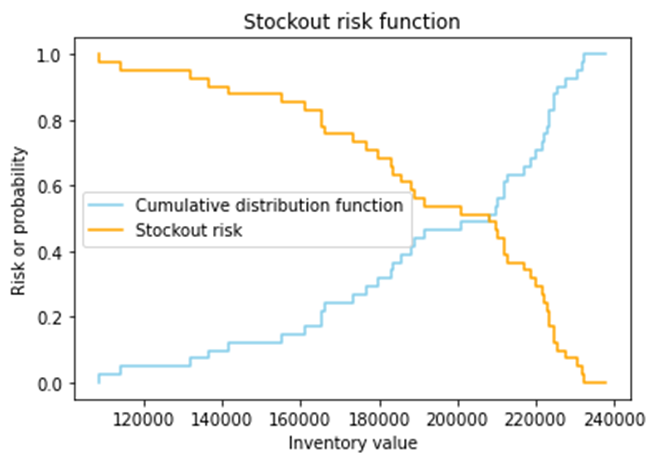
\includegraphics[width=0.9\textwidth]{SectionWarehouses/design_figures/fig_stockout.png}
\captionsetup{type=figure}
\caption{Cumulative distribution function of I(t), and stockout risk function.}
\label{fig_stockout}
\end{figure}

It is necessary to remark that the aforementioned procedure uses one observation of the $I_i(t)$, i.e. the only observed for a part $i$. By extracting the features of the function $I_i(t)$ it is possible to bootstrap $I_i\left(t\right)$, obtaining a probabilistic definition of the inventory behaviour of the part $i$.\par

The movement function $M_i(t)$ is defined based on $I_i(t)$, and the outbound movements $M_i^-\left(t\right)=M_i\left(t\right):M_i\left(t\right)<0$ are considered. The mean value $\mu_i^{M^-}$, and the standard deviation $\sigma_i^{M^-}$ of the quantity involved in the $M_i^-(t)$ are defined. The mean interarrival time $\mu_i^{M_{int}^-}$, and its standard deviation $\sigma_i^{M_{int}^-}$ are defined as well. At this stage, Montecarlo simulation is used to bootstrap a multitude of inventory functions $I_i^{boot}(t)$. Depending on the demand pattern of the part $i$ (see section \ref{secDemandPatterns} for the classification), a different approach is used. When the part $i$ is intermittent, or lumpy a Poisson distribution (see Section \ref{secPoisson}) is used to generate the time instant when there is outbound demand  with $\lambda$ equal to the number of movements of $M_i^-\left(t\right)$:

\begin{equation}
    t \sim Poisson(\lambda = card\{M_i^-\left(t\right)\})
\end{equation}

When parts are erratic or stable, a Gaussian distribution generates the waiting time between the arrivals, using the parameters from the interarrival distribution:

\begin{equation}
    t \sim Normal (\mu=\mu_i^{M_{int}^-},\ \sigma=\sigma_i^{M_{int}^-})
\end{equation}

The quantities of the ${M_i^-}^{boot}\left(t\right)$ are always generated by using a Gaussian function:

\begin{equation}
    {M_i^-}^{boot}\left(t\right) \sim Normal(\mu=\mu_i^{M^-},\ \sigma=\sigma_i^{M^-})
\end{equation}

Algorithm \ref{algo_inventory_bootstrap} identifies the pseudocode  to bootstrap inventory functions.\footnote{The source code to estimate the inventory of a storage system is available \href{https://github.com/aletuf93/logproj/blob/master/logproj/information_framework.py}{here}.}.

\begin{algorithm}[H]
\DontPrintSemicolon
\SetAlgoLined
Consider the movement function $M_i(t)$ of a part $i$\;
Set $\mu_M$ to the mean of $M_i(t)$\;
Set $\sigma_M$ to the standard deviation of $M_i(t)$\;
Set $\mu_M^{int}$ to the mean of the interarrival time of $M_i(t)$\;
Set $\sigma_M^{int}$ to the standard deviation of the interarrival time of $M_i(t)$\;
Set $B$ to the numer of iterations \;
\For{$b:1 \rightarrow B $}{
    \If {Demand pattern of $i$ $\in$ $\{ 'Intermittent', \ 'Lumpy' \}$}
        {$t_{outbound} = \{ Poisson(\lambda=ADI_i)\}$}\;
    
    \If {Demand pattern of $i$ $\in$ $\{ 'Erratic', \ 'Stable' \}$}
        {$t_{outbound} = \{ t \ spaced \ by \ Normal(\mu_M^{int}, \sigma_M^{int})\}$}\;
    
    
    $Quantity_{out} = Normal(\mu_M, \sigma_M)\}$ \;
    Infer the inventory function$I(t)$\;
    Save $\mu_{I(t)}^{b}$\;
    Save $\sigma_{I(t)}^{b}$\;
    Save $min\{I(t)\}^{b}$\;
    Save $max\{I(t)\}^{b}$\;
    
    }
Extract the statistics of $\mu_{I(t)}^{B}$, $\sigma_{I(t)}^{B}$, $min\{I(t)\}^{B}$, $max\{I(t)\}^{B}$.
    
\caption{Bootstrap algorithm for inventory functions.}
\label{algo_inventory_bootstrap}
\end{algorithm}

By considering the minimum, maximum and average value across all the bootstrapped inventory functions, it is possible to make decisions on the target inventory level.

\section{Choice of the storage technology (P2)} \label{secWhTech}

Different storage technologies exist, offering a wide range of solution to stock SKUs. A non-exhaustive list of storage technology involves (see Figure \ref{fig_storageSystem}):

\begin{itemize}
    \item Block stacking. Unit loads are placed on the floor, and eventually stacked ~\cite{Accorsi2017b, Goetschalckx1991, Nishi2010}.
    \item Pallet Racks. Unit loads are placed on different levels by using fixed racks ~\cite{Azadivar1989, Bassan1980, Bortolini2015a, Cardona2013, Roberts1972, Thomas2013}.
    \item Drive-in Pallet Racks. Unit loads are placed side-by-side on racks. Forklifts can travel through the racks. Last-In-First-Out (LIFO) policy is used since unit loads in the back are blocked by the unit loads on the front ~\cite{Manzini2016}.
    \item Push-Back Pallet Racks. Unit loads are placed by pushing back the unit loads already on the racks. LIFO policy is used.
    \item Movable Pallet Racks. Racks can be moved on trails to improve the space utilisation of the warehouse.
    \item Cantilever Racks. These racks are used to store oversize SKUs as metal or wooden bars.
    \item Manual Shelves. These racks host cartons or parts and are served by manual operators.
    \item Automated vertical warehouse. 
    \item Carousel. It is an automates storage system where racks or shelves rotates along a track ~\cite{Hua2008, Hwang1994, Lee1988, Vickson1998}.
    \item Miniload. These systems are fully automated and host cartons or single parts placed inside bins. Bins are automatically stored and retrieved by the cranes of the miniload.
    \item Automated Storage \& Retrieval System (AS/RS). These systems works similarly to miniloads, but managing full-pallet ~\cite{DeKoster2007, Karasawa1980, Manzini2006b, Regattieri2013, Rosenblatt1993, Tappia2015}.
    \item Highly automated robotic warehouse. These systems use shuttles and robots able to move and stack bins containing carton or single parts. All the bins compose a cube with a high storage density, whose storage operations are fully managed by the robots ~\cite{Lerher2016}.

\end{itemize}

% INSERT fig_storageSystem
\begin{figure}[hbt!]
\centering
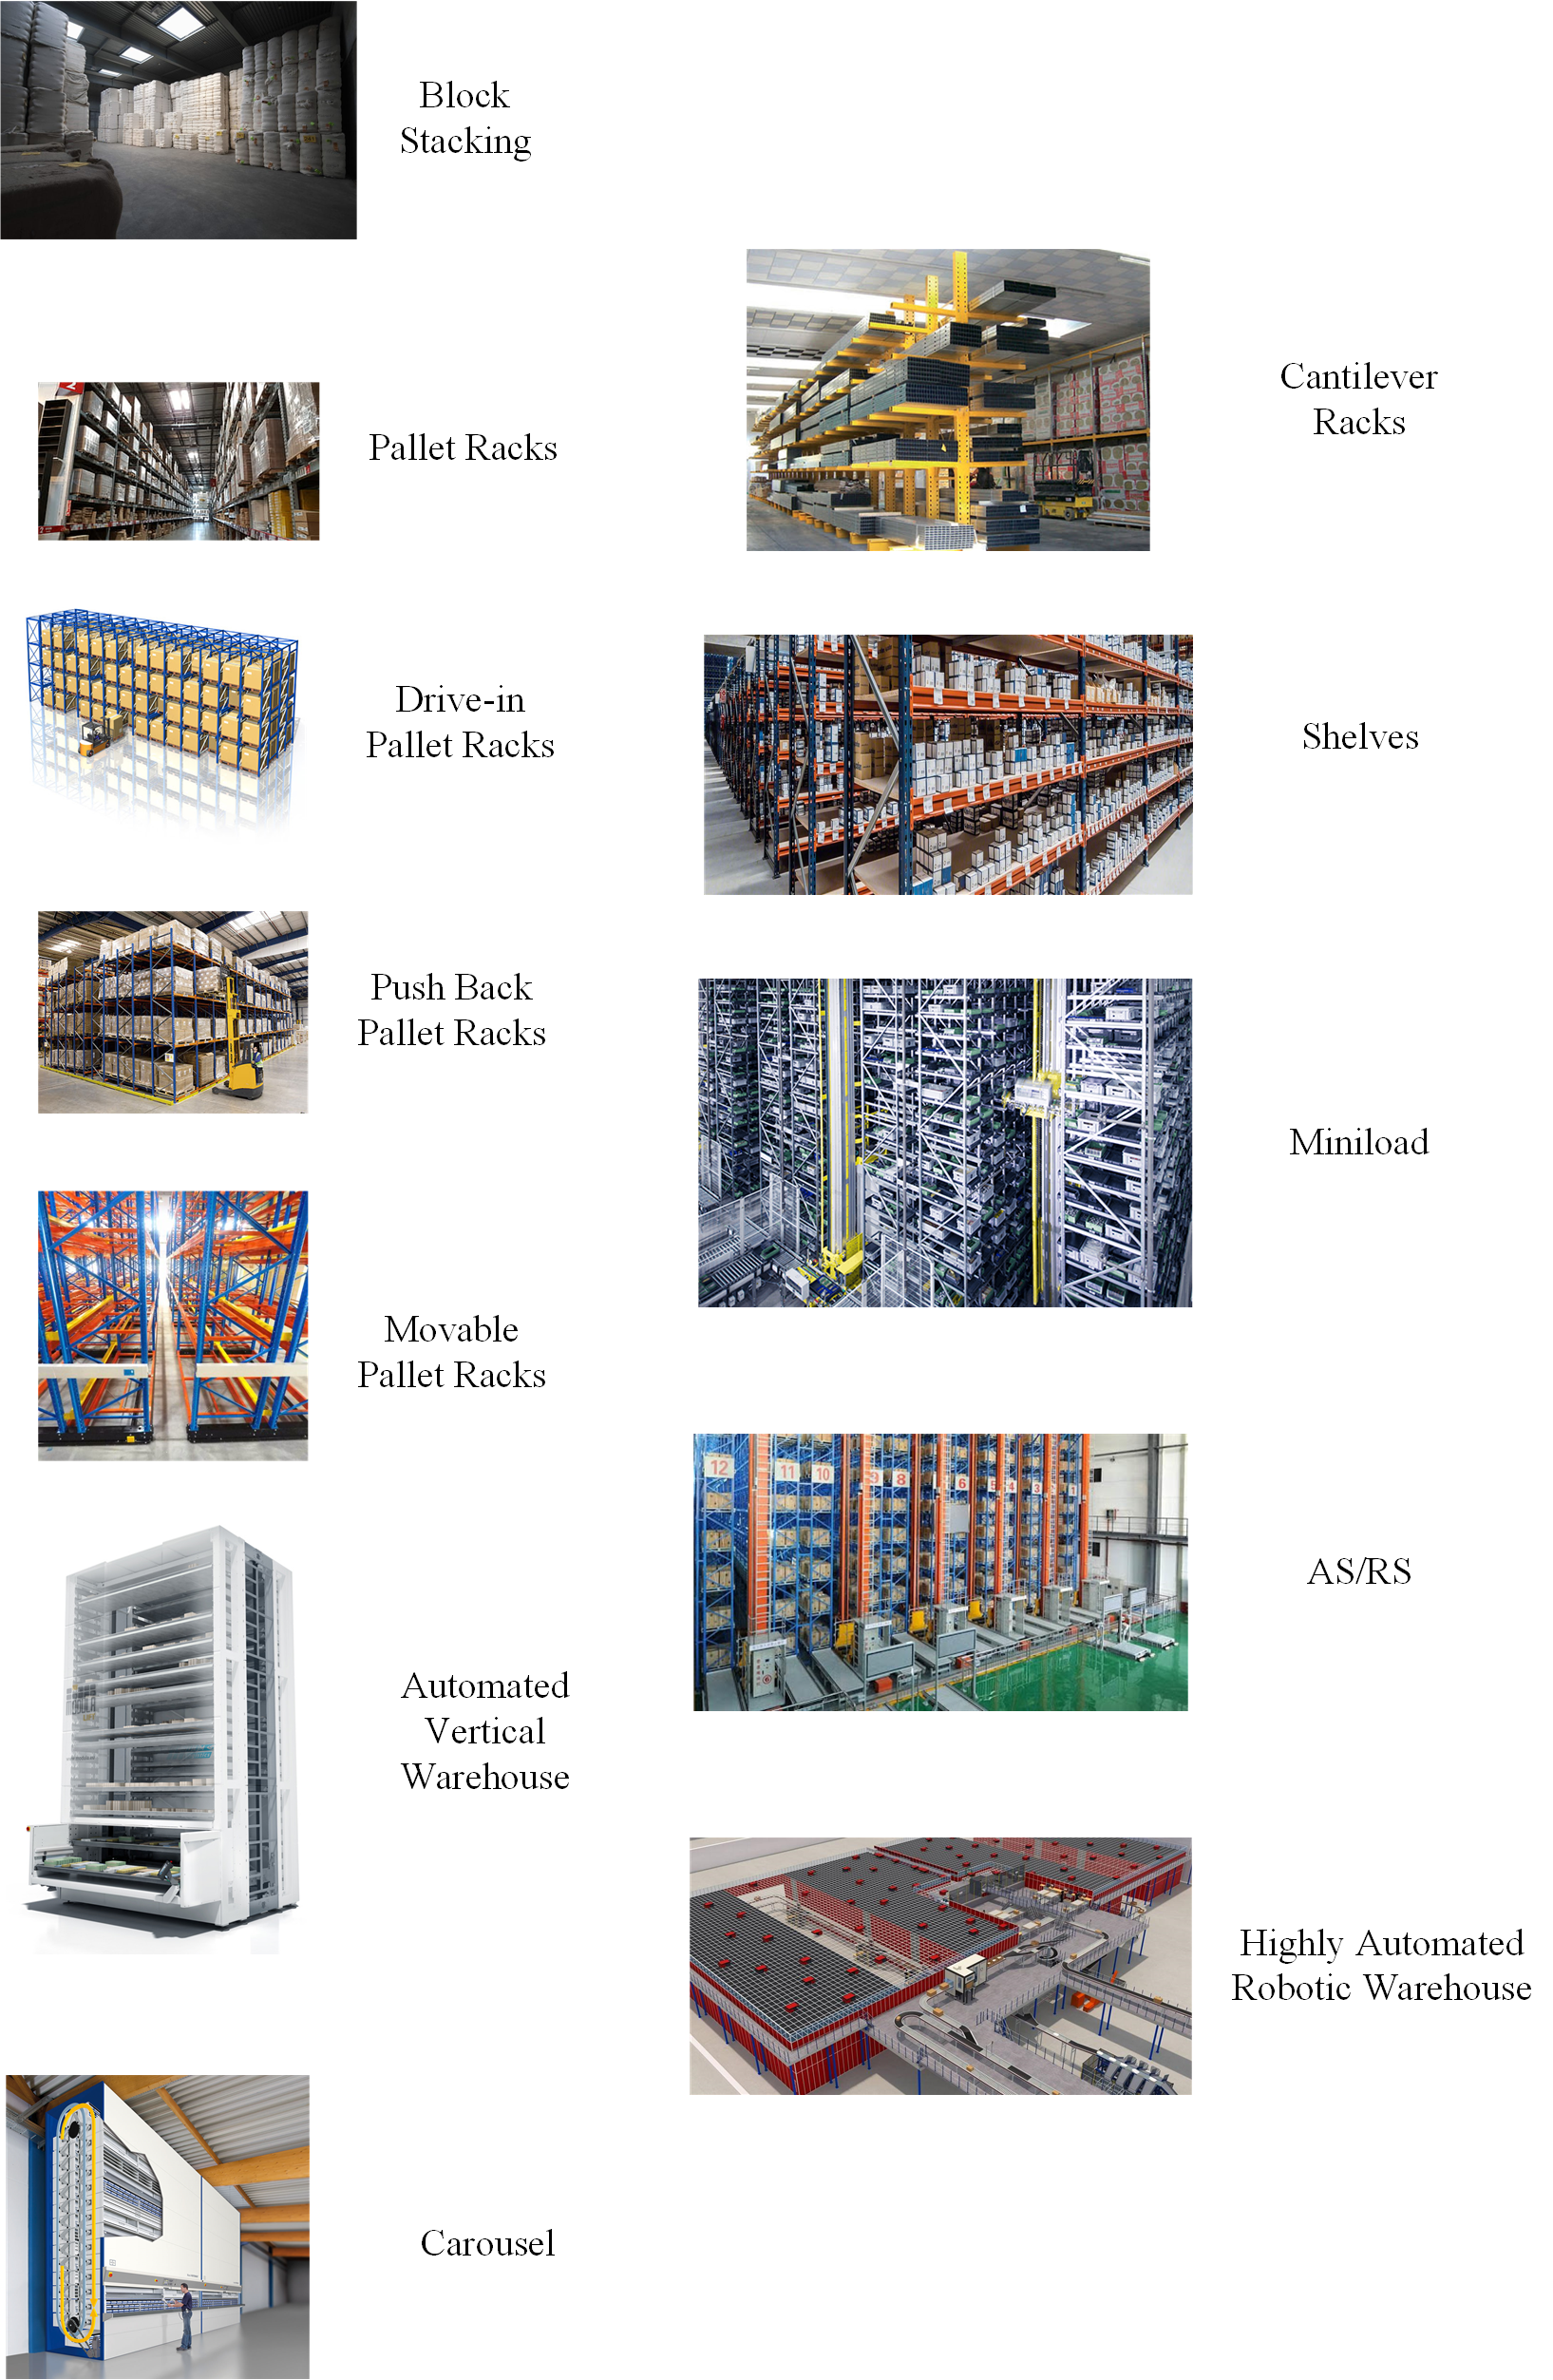
\includegraphics[width=0.9\textwidth]{SectionWarehouses/design_figures/fig_storageSystem.png}
\captionsetup{type=figure}
\caption{Classification of storage technologies.}
\label{fig_storageSystem}
\end{figure}

\clearpage

The different storage technologies are integrated with different storage vehicles to put away and pick the SKUs. A non-exhaustive list of vehicles comprises (see Figure \ref{fig_vehicles}):

\begin{itemize}
    \item Forklift. The traditional handling vehicle used to move any type of SKUs in most of the industries.
    \item Side loader. Handling vehicle able to enter storage racks with narrow aisles.
    \item Pallet Jack. A manual handler to move one pallet at the time.
    \item Walkie Stacker. A forklift used for picking where the operator can stand an move together with the vehicle.
    \item Order picker. A vehicle able to bring a man on the higher levels of the storage system to permit manual picking ~\cite{Taylor2007}.
    \item Crane. The automated crane of an AS/RS or a miniload.
    \item Shuttle. The automated robots of a highly automated storage system
    \item Operator. Manual operators can walk through racks or shelves performing manual picking operations.
    \item AGV forklift. Automated guided forklift able to autonomously put away and pick pallets.
    \item AGV shuttle. Automated guided shuttle able to autonomously move shelves.

\end{itemize}


% INSERT fig_vehicles
\begin{figure}[hbt!]
\centering
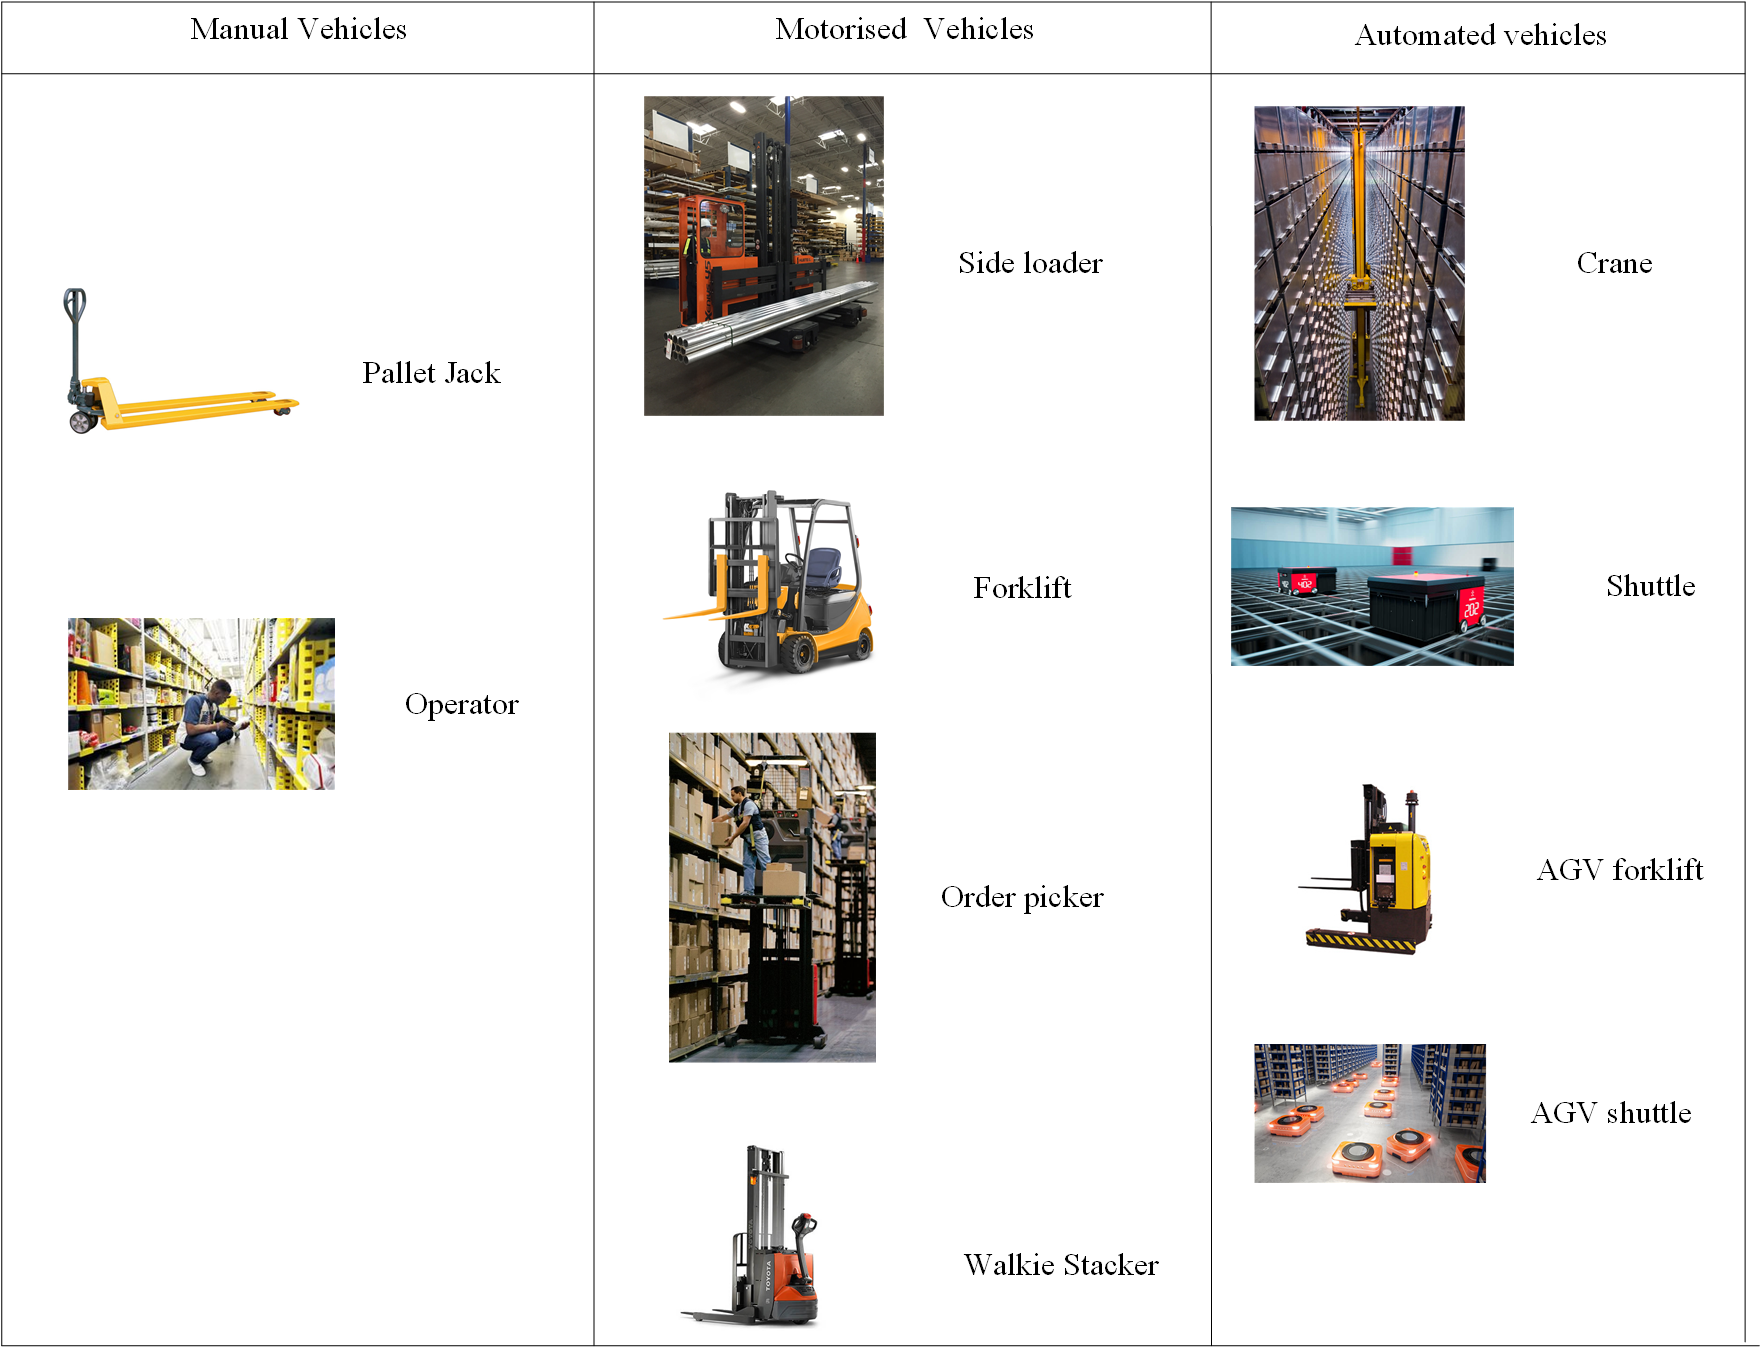
\includegraphics[width=0.9\textwidth]{SectionWarehouses/design_figures/fig_vehicles.png}
\captionsetup{type=figure}
\caption{Classification of handling vehicles.}
\label{fig_vehicles}
\end{figure}

\clearpage

Storage technologies and vehicles can be classified together depending on their degree of flexibility and automation. Figure \ref{fig_technologies} illustrates this classification.

% INSERT fig_technologies
\begin{figure}[hbt!]
\centering
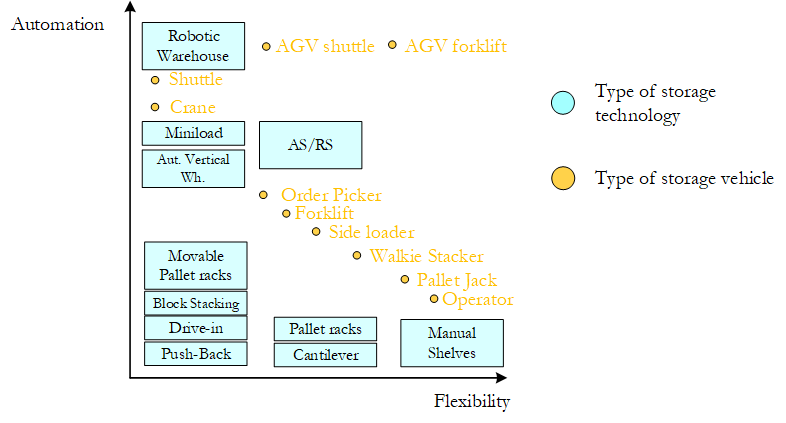
\includegraphics[width=0.9\textwidth]{SectionWarehouses/design_figures/fig_technologies.png}
\captionsetup{type=figure}
\caption{Classification of storage vehicles and storage technologies depending on the degree of automation and flexibility.}
\label{fig_technologies}
\end{figure}

\subsection{Model-driven methods (D4)}
The choice of storage technology is the most challenging decision in the design of a storage system. There is no specific model to assist the decision-maker in this choice. In addition, there are a number of elements to take into account:

\begin{itemize}
    \item the expected throughput;
    \item the available space;
    \item the space saturation of each technology;
    \item the risk due to fragile or inflammable SKUs;
    \item the dimension (i.e. size, and weight) of the SKUs and their stackability;
    \item the economic investment.

\end{itemize}

Generally, discrete event simulation is the preferred way to assess the behaviour of each storage technology, and identify the most suitable one. It is important to remark that a storage node may host multiple storage technologies to deal with different SKUs and to reach different levels of performance.

\section{Storage allocation (P5)} \label{secWhAllocation}
Storage allocation procedures define the space of the storage system to allocate to each SKU ~\cite{Bartholdi2008, Battista2014, Bottani2012, Guerriero2015, Hassini2008, VanDenBerg1998, Walter2013, Yu2015}. In particular, storage systems can be organised using:

\begin{itemize}
    \item a \textit{fast pick} area (FPA) (also known as “forward area”) placed at the ground level of the storage system, where pickers can immediately pick SKUs without wasting time to reach the higher levels of the storage system;
    \item a \textit{reserve} area (RA) storing additional SKUs for all the SKUs in the fast pick area, and all the other SKUs (not in the fast pick area).

\end{itemize}

Storage allocation aims at defining when an FPA is needed, which SKUs should be placed in the FPA, and in which amount ~\cite{Walter2013}. In storage system with multiple technologies, a storage block with a faster technology (e.g. a miniload or a cross-docking area) can be the FPA of a slower reserve storage area (e.g. a drive-in) ~\cite{Hackman1990, Li2009}.\par

The methods for the definition of the inventory level already defined a recommendable amount $I_i$ of an SKU $i$ to keep inhouse. This is the starting parameter for the storage allocation of a greenfield storage system. An inventory snapshot is considered, when dealing with the re-allocation of an existing warehouse, instead. \par

We already introduced the difference between full pallet, carton, and part picking. The package type of the unit load guides the choice of the storage system. A storage system of full pallet does not need allocation since the benefit provided by an FPA is relevant when the number of picks $p_i$ in the FPA is higher than the number of restocks $r_i$ from the RA to the FPA. This condition can be verified when the picking process involves single parts or carton, but never when picking operations are full pallet. In addition, it is important to remember that the RA always hosts full pallet. These pallets are moved down to the FPA and opened to allow carton or parts picking. For each SKU $i$ in the FPA, it is recommendable to have at least the space of two pallets. Otherwise, having a single pallet space in the FPA, it would not be possible to move a pallet from the RA before the pallet in the FPA is completely empty. It is straightforward that SKUs with a $I_i$ lower than two pallets cannot enter the FPA.

\subsection{Model-driven methods (PS4)}
Allocation problem is solved using a model. Re-allocation of a storage system profoundly change the use of the space within the storage system, and it is hard to have observations of any possible configuration to use a data-driven model. We define, first the theoretical amount of space $v_i$ to allocate in fast-pick for each SKU $i$. Secondly, depending on the availability of space, we consider which SKU can enter the FPA. \par

Generally, not all the SKUs of a warehouse are suitable for the FPA. To define which SKUs are suitable to be stored in the FPA we can consider a ranking index, for example, the top 20\% moving based on the $Pop_i$ Pareto curve (see section \ref{secDataDrivenAnalysisWh}. We can think this problem as an instance of the knapsack problem where the FPA has a fixed capacity, and it is filled based on the ranking resulting from the Pareto curve. It is important to remember that this procedure is suboptimal and hard to generalise. The filling heuristics of the knapsack by sorting for a ranking index does not imply the optimality of the solution. In addition, the actual volume to allocate in the FPA is still to be defined. Finally, there are many aspects to be considered. If the inventory levels are low for all the SKUs (e.g. one pallet), it does not make sense to have a fast pick area. Having a fast pick area with a subset of the items must consider the probability to complete an order within the FPA. If this probability is low, implying to retrieve SKUs from the higher levels in order to complete an order, the FPA does not lead to efficiency improvement. Ranking the SKUs on the $OC_i$ could help; nevertheless, there is no optimal policy to define this allocation. Always remember of the rotation frequency of the inventory function $I(t)$ (see section \ref{secDataDrivenAnalysisWh}). The definition of the SKUs worth to be included in the FPA changes with the change of the $I(t)$. \par

The amount of space to allocate to SKU $i$ in the FPA is calculated aiming at minimising the number of restocks $r_i$ between the RA and the FPA. The cost of restocks is the augmented operational cost of setting an FPA; for this reason, it has to be minimised. Let $f_i$ be the annual outbound volume of SKU $i$, and $S$ the total space of the FPA (e.g. given by the sum of the volume of all the locations at the ground floor of the warehouse).\par

It is demonstrated ~\cite{Bartholdi2017} that the value of $v_i$ minimising $r_i$ is:

\begin{equation}
    v_i^\ast=S\left(\frac{\sqrt{f_i}}{\sum_{j}\sqrt{f_j}}\right)
\end{equation}

This optimal (OPT) strategy produces decimal values of $v_i$, that need to be rounded. In addition, this policy can be hard to be applied in practice, since each SKU can have a different space in the FPA. For this reason, two additional strategies are introduced. The equal space (EQS)  strategy allocates the same amount of space for all the SKUS, $v_i=\frac{S}{card\left(SKU\right)}$. An equal time (EQT) strategy, defines the volume for each SKU $i$, such that all the SKUs have the same number of restocks $r_i$ (i.e. all restocks have the same frequency), $v_i=S\left(\frac{f_i}{\sum_{j} f_i}\right)$. Table \ref{tab_allocation} identifies the allocated space $v_i$, the number of restocks $r_i$, and the total number of restocks $R=\sum_{i} r_i$.

% INSERT tab_allocation
\begin{figure}[hbt!]
\centering
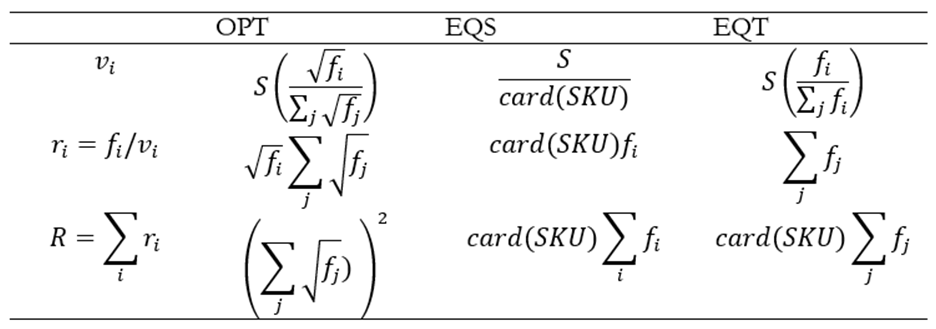
\includegraphics[width=0.9\textwidth]{SectionWarehouses/design_figures/tab_allocation.png}
\captionsetup{type=table}
\caption{Storage allocation policies.}
\label{tab_allocation}
\end{figure}

The OPT strategy should be preferred when possible. Nevertheless, it could be infeasible, from an organisational perspective, to define slots of the FPA with different dimensions. In this case, the EQS strategy should be preferred. In case the restock activity results intense for some SKUs, the EQT strategy allows to restock all the SKUs together (on average) enhancing the planning of the restock activity.

\section{Storage assignment/slotting (P2)} \label{secWhAssignment}
Storage assignment (also known in the literature as \textit{slotting}) aims at defining a storage location for each SKU of the storage system. This activity is fundamental since it heavily affects the travelled distance to put away and pick SKUs during the operations. In practice, three assignment strategies exist \cite{Accorsi2017_stockSafety, Ang2012, Battini2015, Bortolini2015, Cardona2016, Chen2011, Fontana2014, Goetschalckx1990, Guerriero2013, Guo2016, Jarvis1991, Kallina1976, Larson1997, Le-Duc1999, Mallette1972, Malmborg1989, Manzini2015b, MuppaniMuppant2008, Pan2015, Quintanilla2015, Sooksaksun2012, Xie2014}:

\begin{itemize}
    \item random assignment strategy; SKUs are randomly assigned to the storage locations;
    \item class-based assignment strategy; SKUs are clustered into classes, and storage locations are clustered into the same classes. SKUs are randomly assigned within the set of storage locations of their class;
    \item dedicated assignment strategy; each SKU is assigned to specific storage locations.

\end{itemize}

While random assignment strategy does not need any additional model; both model- and data-driven models help in the definition of class-based and dedicated assignment.

\subsection{Model-driven methods (PS3)}
Ranking methods are particularly efficient to deploy a dedicated assignment strategy. In particular, they rank the SKU by considering an SKU profiling index (e.g. the $Pop_i$), and they rank the storage location by summing the distance to travel from the input point to the storage location, to the output point. The two rankings provide the information to fill the storage system in a bin-packing fashion. Starting by placing the SKUs with a high value of the profiling index (e.g. the $Pop_i$) to the locations with a smaller distance value. When a storage location has no space to host SKUs, the following storage location is used. \footnote{The source code to assign SKUs to storage locations is available \href{https://github.com/aletuf93/logproj/blob/master/logproj/P2_assignmentProblem/warehousing_ABC_saving.py}{here}.}.\par

A similar method can be used to define a class-based assignment. A common class-based strategy is called “ABC”, and it is based on the definition of three classes depending on an SKU profiling index (e.g. the $Pop_i$). SKUs with high $Pop_i$ belong to class A, with intermediate $Pop_i$ to class B, with low $Pop_i$ to class C. In practice the ranking of storage locations is used to define a Pareto curve on the value of their distance to the I/O, and to generate the three classes, for example:

\begin{itemize}
    \item the first 20\% of the closest storage locations to the I/O are labelled as class A locations;
    \item the following 30\% of the closest storage locations to the I/O are labelled as class B locations;
    \item the remaining 50\% are labelled as class C locations.

\end{itemize}

At this stage, storage locations are filled with SKUs, based on the ranking on an SKU profiling index, and SKUs inherits their class from the location where they are placed. \par

Both these data-driven methods, highly depend on the frequency of rotation of the inventory function $I(t)$, since after a period of time an SKU can be stored in a wrong position since its SKU profile index changed. For this reason, it is necessary to reconsider the storage assignment periodically. Decision support systems have been developed to support the warehouse managers in this choice ~\cite{Accorsi2014}.

\subsection{Data-driven methods (PS2)}

Data-driven methods provide tools to generate classes of SKUs by clustering them based on recurrent patterns of their features ~\cite{Bindi2009, Brynzer1996, Liu1999, Chiang2013, Moshref-Javadi2016, Pang2017, Smith2012, Xiao2012}.\par

Correlated storage assignment uses an incidence matrix $M_{i,o}$ between SKUs and orders (i.e. ‘1’ if an SKU $i$ has been picked during order $o$; ‘0’ otherwise) to define a proximity matrix $D_{i,j}$ where $i$ and $j$ are SKUs. A similarity index (e.g. the Jaccard index) is used to convert the incidence matrix into a proximity matrix. At this stage, hierarchical clustering is used to define clusters (i.e. classes) of SKUs. The SKUs within the same cluster have been historically picked together. For this reason, they are placed close to each other.\par

Another data-driven method can be used to investigate the degree of health of the assignment strategy of a storage system. It always considers two metrics for each SKU: a profiling index (e.g. the $Pop_i$), and the average distance $D_i$ to reach the SKU (or the average of the distances when an SKU has multiple storage locations). When the assignment is optimal, the two metrics are linked with an exponential law ~\cite{Manzini2018}: $Pop_i=\alpha e^{-\beta D_i}$. During the operations of the warehouse, with the rotation of the frequency of the inventory function, the link between the two functions becomes similar to a Gaussian function (see Figure \ref{fig_layout_profile}). \par

By considering the gap between these two functions, the cost saving of exchanging locations between locations can be measured.\footnote{The source code to estimate the saving obtained by exchanging the position of two storage locations is available \href{https://github.com/aletuf93/logproj/blob/master/logproj/P6_placementProblem/warehouse_graph_definition.py}{here}.}

\section{Layout design (P6)}
Layout design deeply affects the total travelled distance of a storage system ~\cite{Jaimes2012, Le-Duc1999, Pliskin1982, Tutam2015, Zhang2002}. A storage system is generally composed of different storage blocks, with different storage technologies (identified in Section \ref{secWhTech}). For this reason, the storage allocation and assignment (Section \ref{secWhAllocation} and section \ref{secWhAssignment}) can be repeated for the SKUs assigned to each storage block.

\subsection{Model-driven methods (PS3)}
At this stage, the layout design procedure produces a number of blocks with different technologies, of performing different activities (e.g. picking, packing, quality control), which need to be placed within the same building. Plant layout design procedures (see section \ref{secProdLayoutDesign}) applies to identify a feasible placement of the areas minimising the distances between the blocks.\par

It is important to remark that, so far, all the method proposed aims at the minimisation of the travelled distance to pick each SKU within each warehouse block. When designing the entire storage system, it is important to identify the material and information flows between these blocks, and to place them such that they are minimised. Figure \ref{fig_spaghetti_wh} identify the material flows between different areas of the same storage system. Areas with an intense material flow should be placed closed to each other.

% INSERT fig_spaghetti_wh
\begin{figure}[hbt!]
\centering
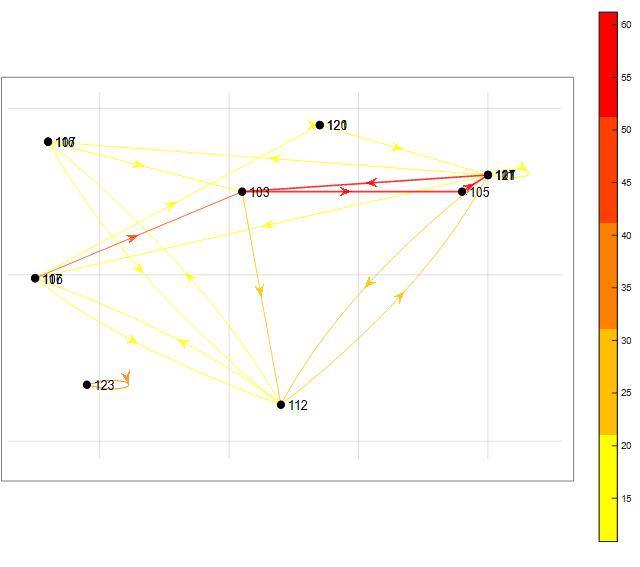
\includegraphics[width=0.9\textwidth]{SectionWarehouses/design_figures/fig_spaghetti_wh.png}
\captionsetup{type=figure}
\caption{Spaghetti chart of a warehouse node.}
\label{fig_spaghetti_wh}
\end{figure}

\subsection{Data-driven methods (D3)}
The spaghetti chart introduced above is static, and it does not consider the dynamics of the operations of the storage system. To simulate the effect of time on the exchange of materials, a from-to matrix $T$ with entries $t_{j,k}$ is defined accordingly to the intensity of flow exchange between control points (CP), identifying different areas. $t_{j,k}$ estimates the number of trips between CPs $j$ and $k$. The value of $t_{j,k}$ is static and does not consider how the system evolves. Nevertheless, it gives no information on the work in progress (WIP) between CPs (i.e. the number of SKUs waiting to be processed/shipped), that is an important parameter for the design of the buffering areas. A Markow Chain (MC) is introduced (see \ref{secMarkovChain}) to estimate this parameter. An MC applies statistical Markov properties on a directed graph to measure the probability of occurrences of an event (i.e. the node) given the probability of the transitions between the events (i.e., the arcs). In this case, $T$ is the input matrix representing the probability of transitions between the events. A complete graph $G\left(V,E\right)$ is defined as follows.

\begin{itemize}
    \item a set of nodes, corresponding to the number of rows of the matrix (i.e. each CP is a node of $G$);
    \item a set of directed arcs representing the probability of transition between the nodes (i.e., the CPs). The weight of each arc represents the probability that the edge is travelled to transfer materials. This value is calculated as: ${\hat{t}}_{j,k}=\frac{t_{j,k}}{\sum_{j}^{n}\sum_{k}^{n}t_{j,k}}$
\end{itemize}

The value of ${\hat{t}}_{j,k}$ defines the probability of a transition from CP $j$ to CP $k$. MC implements an initial state of the system (i.e., a number of SKUs located in each CP) and it simulates a given number of transitions.  The transitions redistribute the initial state value among the others CPs according to the transition probability ${\hat{t}}_{j,k}$. The initial state of the MC is chosen accordingly to the specifics of the real storage system (e.g., the inbound node is fully loaded, and all the others are empty) and a number of transitions on the graph are performed to check how the WIP is redistributed after a number of transitions of the system. Figure \ref{fig_markovChain_wh} illustrates the outcome of a MC after a number of iterations, i.e. the probability to find WIP at each CP.

% INSERT fig_markovChain
\begin{figure}[hbt!]
\centering
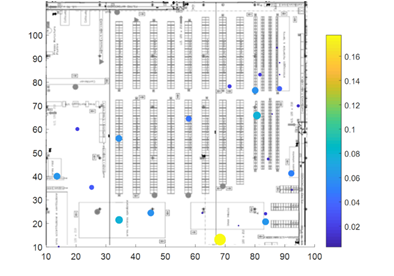
\includegraphics[width=0.9\textwidth]{SectionWarehouses/design_figures/fig_markovChain.png}
\captionsetup{type=figure}
\caption{Markov chain outcome to estimate the work in process (WIP) at each control point (CP).}
\label{fig_markovChain_wh}
\end{figure}

Even if this approach does not provide statistics on the number of SKUs in each buffering areas, it defines how the workload flows between control points. Some CPs have a higher probability of hosting WIP after a significant number of transitions. This fact suggests that these CPs deserve much more area than the others. DES can be used to accurately design these CPs (see section \ref{secWhAreaDesign}).

\section{Picking policy design (P7)}

Depending on the type of technology involved in a storage system, it can be necessary to design a picking policy to connect the different storage blocks ~\cite{Bartholdi1996, Choe1991, Ene2012, Jarvis1991, Lin1999, Marchet2015, Petersen2004, Roodbergen2015, VanGils2017}. Fully automated storage technologies (e.g. AS/RS, miniload and shuttle systems) automatically manage both the assignment and the picking strategy actuated by the automation. Manual storage systems (shelves, racks, stacking areas) need policies for pickers to complete the orders. In addition, it is rare to find fully automated storage systems. For this reason, at some stage of the process, the parts picked by automated systems need to be consolidated with the others.\par

Picking policies are implemented only for the outbound activities, since they are generally responsible of the majority of the workload of a storage system:

\begin{itemize}
    \item single-order: the picker receives a single picking list with a single order. He/she travel across all the storage system to pick the parts of the order;
    \item multi-order with batching: the picker receives a single picking list with multiple order. She/he is equipped with tools (e.g. a cart with slots, or a put-to-light cart) to pick parts belonging to different orders. Parts remain separated during the whole picking process, and the orders are complete at the end of the route or the picker ~\cite{Chen2005a, Valle2017, Zulj2018};
    \item multi-order with zoning: Pickers are assigned to a specific zone of the storage system (i.e. a subset of storage locations). A picker receives a single picking list with multiple orders. He/she is equipped with tools (e.g. a cart with slots, or a put-to-light cart) to pick parts belonging to different orders. Parts remain separated during the whole picking process, and the orders are completed in the outbound area by aggregating the subset of parts picked from each zone;
    \item multi-order with zoning and sorting: Pickers are assigned to a specific zone of the storage system (i.e. a subset of storage locations). A picker receives a single picking list with multiple orders. Parts are collected together and separated after the picking process in a sorting zone close to the outbound area.

\end{itemize}

\subsection{Model-driven methods (D4)}
Discrete event simulation (DES) is the method used to compare the efficiency of different picking policies applied to the same storage system ~\cite{Caron2007, Lu2016}. DES allows to estimate the efficiency of each policy and to identify bottlenecks of the process. 

\section{Route design (P3)}

Storage systems can be very congested areas with hundred of operators travelling to put away and pick parts. For this reason, as for the roads where we are used to riding our bicycles, precise policies exist ~\cite{Caron2007, Petersen1999, Roodbergen2001, Roodbergen2006}:

\begin{itemize}
    \item return policy: allows to travel the aisles and corridors (i.e. the edges of the set $E$) of the storage system in both their directions;
    \item traversal policy: allow to travel the aisles and corridors (i.e. the edges of the set $E$)  of the storage system in one direction (one way).
\end{itemize}


\section{Inbound and outbound area design (P5)} \label{secWhAreaDesign}

This phase aims at designing handling (i.e., buffering or processing) areas. In the handling areas, the operators prepare the SKUs for storage (e.g., inbound, inspection) or shipping (e.g., packing, order consolidation) ~\cite{Bassan1980, Heragu2005b, Pandit1993}. Buffering areas are zones between activities where the SKUs wait for handling. The design of the buffering area is crucial since too small areas would generate congestions of the activities. Otherwise too large areas remove space from the storage/handling areas

\subsection{Model-driven methods (D4)}

To get statistics on the expected workload in this area, discrete event simulation (DES) is used. Typically, inbound and outbound areas deserve design validation via simulation due to their importance for all the receiving/shipping processes. Figures \ref{fig_DES_inboud} and \ref{fig_DES_outbound} illustrates the flowchart of a DES model and the data needed to support the design of these areas. 


% INSERT fig_DES_inboud
\begin{figure}[hbt!]
\centering
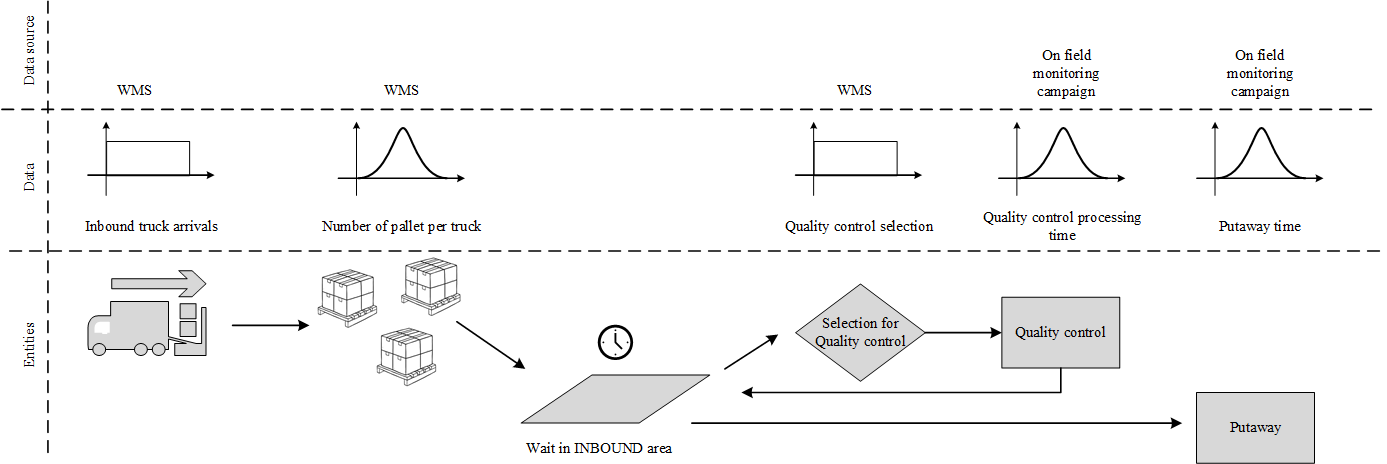
\includegraphics[width=0.9\textwidth]{SectionWarehouses/design_figures/fig_DES_inboud.png}
\captionsetup{type=figure}
\caption{Discrete event simulation (DES) of the inbound processes of a storage system.}
\label{fig_DES_inboud}
\end{figure}

% INSERT fig_DES_outbound
\begin{figure}[hbt!]
\centering
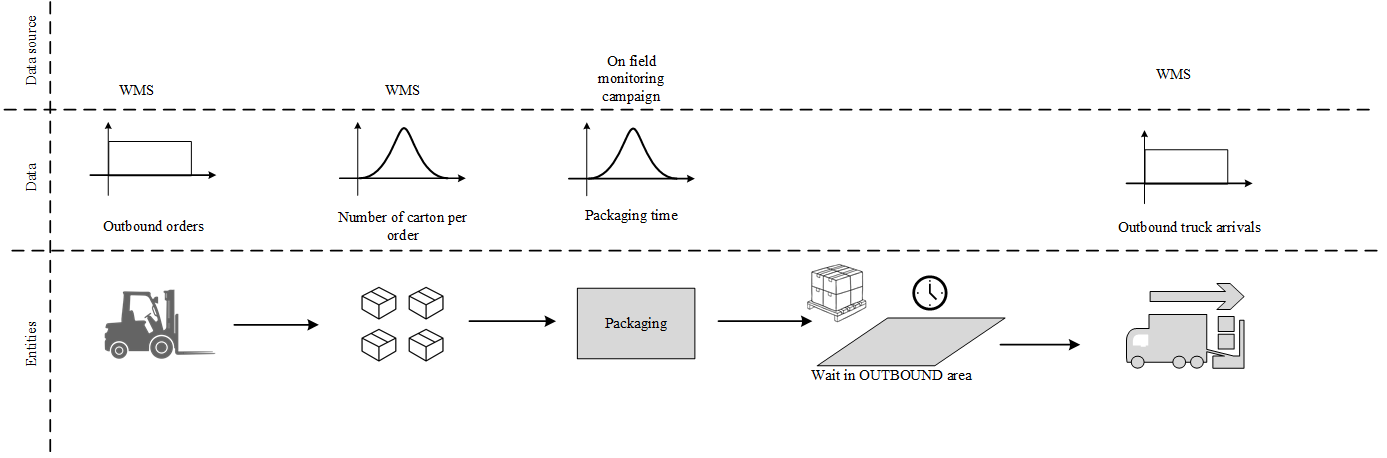
\includegraphics[width=0.9\textwidth]{SectionWarehouses/design_figures/fig_DES_outbound.png}
\captionsetup{type=figure}
\caption{Discrete event simulation (DES) of the outbound processes of a storage system.}
\label{fig_DES_outbound}
\end{figure}

It is necessary to have data about the probability distribution of the execution time of the tasks, to feed the DES properly. Considering the inbound process, it is necessary to know the distribution of the arrivals of trucks and the distribution of the number of pallets transported by each truck. The arrivals distribution is usually available from the warehouse management system (WMS); otherwise, a random distribution over the daily shift can define their arrival time. After truck unloading, pallets wait in the inbound area (the one to be designed) for the following processes. It is necessary to know the distribution of the execution time for each of the following processes and to know the number of resources dedicated to these activities. On-field monitoring campaign aims at collecting these data. \par

Outbound modelling is similar to the inbound modelling process. To design outbound areas, it is necessary to know the distribution of arrivals of the shipping trucks, and the distribution of picking and packing times. These values can be obtained, as well, via the on-field monitoring campaign or by analysing the records of the WMS.\par

The DES produces charts of the WIP at each control point. Figure \ref{fig_DES_WIP} illustrates an example of the number of pallet waiting at the inbound and outbound area of a storage system.\par

% INSERT fig_DES_WIP
\begin{figure}[hbt!]
\centering
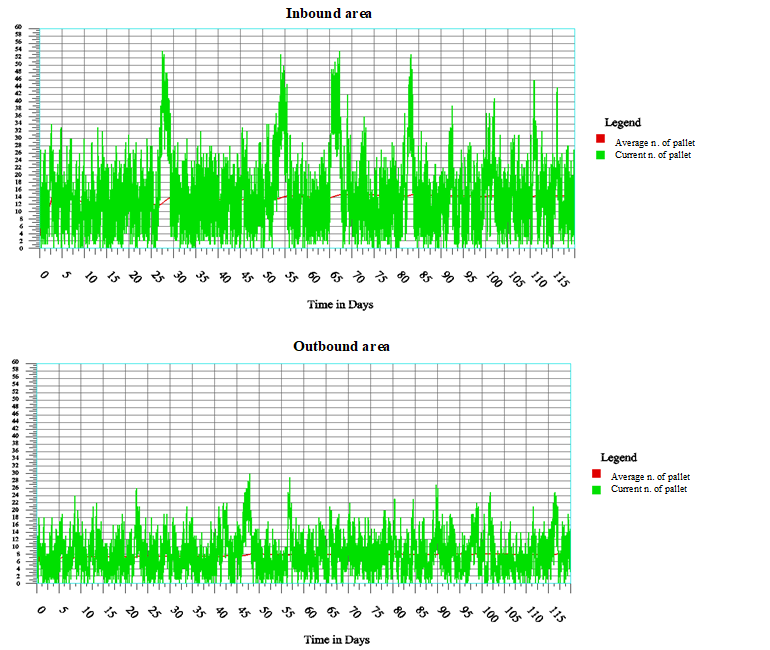
\includegraphics[width=0.9\textwidth]{SectionWarehouses/design_figures/fig_DES_WIP.png}
\captionsetup{type=figure}
\caption{Work in process (WIP) time series of the inbound and outbound areas of a storage system.}
\label{fig_DES_WIP}
\end{figure}

At this stage, each storage and handling area is adequately designed and accounts for a precise area ($m^2$) on the plant layout. Areas should be, then, placed on the available space such that CPs which exchange intense materials flows are close to each other.









%\clearpage
\bibliographystyle{ieeetr}
\bibliography{SectionWarehouses/design_ref}
